\documentclass[10pt,a4paper]{article}
\usepackage[utf8]{inputenc}
\usepackage[T1]{fontenc}
\usepackage{polski}
\usepackage{lmodern}
\usepackage[a4paper,margin=1.9cm]{geometry}
\usepackage{amsmath,amssymb}
\usepackage{graphicx}
\usepackage{booktabs,longtable,tabularx,array}
\usepackage{caption}
\usepackage{microtype}
\usepackage{xcolor}
\usepackage{enumitem}
\usepackage[colorlinks=true,linkcolor=blue,urlcolor=blue]{hyperref}
\emergencystretch=3em
\captionsetup{font=small,labelfont=bf}
\setlength{\parskip}{3pt}
\setlength{\parindent}{0pt}
\setlist{itemsep=1pt,topsep=2pt}
\newcommand{\LdepRodfourzero}{-17.7}
\newcommand{\LdepRodfive}{-2.1}
\newcommand{\LdepSphfourzero}{-45.6}
\newcommand{\LdepSphfive}{-5.4}
\newcommand{\LegKnowlesfourzero}{+15.3}
\newcommand{\LegObsfourzero}{+14.7}
\newcommand{\LknSixtwozero}{-3.7}
\newcommand{\LknSixfourzero}{+4.1}
\newcommand{\LknSixfive}{-0.8}
\newcommand{\LknThirtyFivetwozero}{-3.7}
\newcommand{\LknThirtyFivefourzero}{+4.1}
\newcommand{\LknThirtyFivefive}{-0.8}
\newcommand{\LknqSixtwozero}{-5.9}
\newcommand{\LknqSixfourzero}{+1.7}
\newcommand{\LknqSixfive}{-1.2}
\newcommand{\LknqThirtyFivetwozero}{-5.9}
\newcommand{\LknqThirtyFivefourzero}{+1.7}
\newcommand{\LknqThirtyFivefive}{-1.2}
\newcommand{\LminSix}{-6.1}
\newcommand{\LminThirtyFive}{-5.0}
\newcommand{\LobsSixtwozero}{-3.5}
\newcommand{\LobsSixfourzero}{+1.4}
\newcommand{\LobsSixfive}{-2.3}
\newcommand{\LobsThirtyFivetwozero}{-4.4}
\newcommand{\LobsThirtyFivefourzero}{-0.3}
\newcommand{\LobsThirtyFivefive}{-2.6}
\newcommand{\LpegTwoKnowlesfourzero}{+13.3}
\newcommand{\LpegTwoObsfourzero}{+13.6}
\newcommand{\LsaltHifourzero}{-18.0}
\newcommand{\LsaltHifive}{-1.4}
\newcommand{\LsaltLofourzero}{-4.6}
\newcommand{\LsaltLofive}{-0.4}
\newcommand{\LxFivePEG}{+1.2}
\newcommand{\LxFortyPEG}{+15.1}

\newcommand{\PT}{\textsuperscript{[PT]}}
\newcommand{\ABS}{\textsuperscript{[ABS]}}
\newcommand{\dG}{\Delta\Delta G}
\usepackage{etoolbox}
\newcommand{\citone}[1]{\citsep\ref{#1}\gdef\citsep{,\,}}
\newcommand{\cit}[1]{[\gdef\citsep{}\forcsvlist{\citone}{#1}]}

\title{Przegląd literatury pod kątem naszych pytań:\\
\large hybrydyzacja 13 bp w EG/PEG, preferencyjne oddziaływania, sól, deplecja, barwniki}
\author{Notatki źródłowe: \texttt{analysis/literature\_check/notes/Q*.md}}
\date{9 października 2026; sekcja Q8: 11 października 2026}

\begin{document}
\maketitle
\vspace{-1.6em}

\textbf{Sposób pracy.} Pięć niezależnych przeszukiwań (Q1; Q2; Q3; Q4+Q7; Q5+Q6). Każdy DOI sprawdzono w Crossref API (wyjątek: IJCCE 2020, sprawdzony przez doi.org i stronę wydawcy). Oznaczenia: \PT{} pełny tekst przeczytany, \ABS{} tylko abstrakt; liczby podaję wyłącznie z pełnych tekstów, chyba że zaznaczono inaczej. Strony ACS, RSC i Elsevier były dla skryptów zablokowane, więc część kluczowych prac znamy tylko z abstraktu (lista w sekcji~\ref{sec:ogr}). Pobrane PDF-y OA są w \texttt{literature/review\_2026-10/} (podfoldery \texttt{q2/}, \texttt{q4\_q7/}, \texttt{q5\_q6/}). Obliczenia: \texttt{analysis/literature\_check/*.py}.

\section*{Co to zmienia dla naszej pracy}
\begin{enumerate}[leftmargin=*]
\item \textbf{Empiryczne m-wartości Knowlesa \cit{b:kn11} opisują nasze dane bez dopasowania.} EG 40\%: przewidywane $\LegKnowlesfourzero$ vs zmierzone $\LegObsfourzero$~kJ/mol. PEG 200 40\%: $\LpegTwoKnowlesfourzero$ vs $\LpegTwoObsfourzero$. PEG 35k 20\%: $\LknThirtyFivetwozero$ do $\LknqThirtyFivetwozero$ vs $\LobsThirtyFivetwozero$. Różnica jest tylko przy małych stężeniach: przy 5~wt\% mamy $\LobsThirtyFivefive$ wobec $\LknThirtyFivefive$ do $\LknqThirtyFivefive$, czyli nasza stabilizacja narasta 2--3× szybciej (rys.~\ref{fig:budget}).
\item \textbf{W rozcieńczonym roztworze wodnym nie ma akumulacji netto Na$^+$ przy PEG; lokalna koordynacja jest możliwa, ale słaba} (sekcja~\ref{sec:q8}). Wszystkie objętościowe pomiary termodynamiczne (VPO, dyfuzja wieloskładnikowa) dają $\mu_x>0$ dla NaCl i KCl: sól jest wykluczana, a$_\pm$ rośnie, dupleks powinien się \emph{stabilizować}. W rozkładzie na jony Na$^+$ ma $+4.7\pm2$~cal\,mol$^{-1}$(molal EO)$^{-1}$, czyli zero akumulacji \cit{b:kn15}. Bilans $\Gamma_\text{Na}=\Gamma_\text{koord}-\Gamma_\text{wypchn}$ dopuszcza koordynację rzędu $\kappa\approx0.04$~M$^{-1}$ na EO, czyli zgodną z \emph{dolną} wartością z naszego DOSY (0.055), ale nie z górną (0.17) ani z $\kappa=0.49$ z Bielec 2022 \cit{b:bielec22} ($-290$~cal). Nawet przy prawdziwej koordynacji $K$ zależy od a$_\pm$ netto, więc kanał solny stabilizuje. \textbf{Najmocniejszy argument za akumulacją Na$^+$ w wodzie} pochodzi z naszych danych: nadmiarowe spowolnienie Na$^+$ w DOSY dla PEG $\ge$1000 ma ten sam znak przy każdej poprawce lepkościowej i pojawia się progowo z długością łańcucha (EG i PEG 200: zero), jak przy chelatowaniu wieloma grupami EO. Słabość: DOSY mierzy ruchliwość, a nie aktywność, i nie widzi członu wykluczenia.
\item \textbf{Dowody „wiązania” Na$^+$/K$^+$ są tym silniejsze, im pośredniejszy pomiar i im mniej wody.} Wiązanie jest prawdziwe w ciele stałym, w rozpuszczalnikach organicznych, na żywicach, na granicy woda/nitrobenzen i w nanoporach przy 1--4~M soli. W wodzie objętościowej termodynamika daje $\approx0$, transport (DOSY) $-30$ do $-100$, a wnioskowanie z $K$ hybrydyzacji $-290$~cal (rys.~\ref{fig:q8}). Nawet w nanoporze energia na monomer jest mała (0.03--0.27~kT); „naładowany PEG” wynika z sumowania po kilkudziesięciu monomerach. Po czterech latach nikt niezależnie nie potwierdził kompleksowania z Bielec 2022: z 9 prac cytujących 4 to autocytowania lub IChF, a jedna zewnętrzna przyjmuje mechanizm bez testu \cit{b:silva}.
\item \textbf{Deplecja (granica białkowa) jest liniowa w stężeniu monomerów i niezależna od M} \cit{b:hanke,b:odijk96}, a więc nie nasyca się i nie daje odwrócenia. Liczbowo przy 5~wt\% daje $\LdepRodfive$ do $\LdepSphfive$~kJ/mol (rząd naszego plateau), ale przy 40\% już $\LdepRodfourzero$ do $\LdepSphfourzero$. Sama deplecja nie wyjaśnia kształtu; potrzebny jest człon dodatni rzędu 1.6--3.4~kJ/mol na molal monomeru (preferencyjne oddziaływania wg Knowlesa mają właściwy rząd).
\item \textbf{Bezpośredniego dowodu kontaktu glikol/PEG--zasada w ssDNA lub dupleksie B nie ma.} Brak NOE dla EG i PEG 8000 przy G-kwadrupleksie \cit{b:traj}; dane rozpuszczalności zasad w glikolach (Herskovits 1972 \cit{b:hersk72}) są niedostępne online. Grupa Recorda nie opublikowała zapowiadanych $\alpha$ dla zasad ani $\chi$(rozmiar DNA); w reanalizie podaje $\chi_\infty=0.6\pm0.06$, a nie 0.45 \cit{b:shkel}.
\item \textbf{Stała dielektryczna wnosi najwyżej około 2~kJ/mol} (model PB skalibrowany na naszym nachyleniu solnym; nawet znak zależy od geometrii ssDNA). Wartość $\varepsilon=56.74$ cytowana w SI Bielec 2022 jest obliczona, nie zmierzona \cit{b:panraksa}.
\item \textbf{Barwniki to realne ryzyko systematyczne dla długich PEG.} Stacking Atto488/Atto647N na tym samym końcu daje do około $-2.7$~kJ/mol (różnica tylko około 1.2$\sigma$, \cit{b:bielec20}). Atto647N jest kationowy i silnie hydrofobowy (MIF 1361, \cit{b:hughes}). Jeśli crowder modyfikuje stacking lub adsorpcję akceptora, efekt jest tego samego rzędu co cały $\dG$ długich PEG.
\item \textbf{Znak efektu długiego PEG zależy od soli} (stabilizacja przy niskiej, destabilizacja przy 1 M NaCl: \cit{b:markarian,b:nakano04,b:karimata07}). Nasze 35~mM leży w reżimie stabilizacji. Wyjaśnienie progu (Karimata 2007) jest w pełnym tekście, którego nie mamy.
\end{enumerate}

\begin{figure}[h]
\centering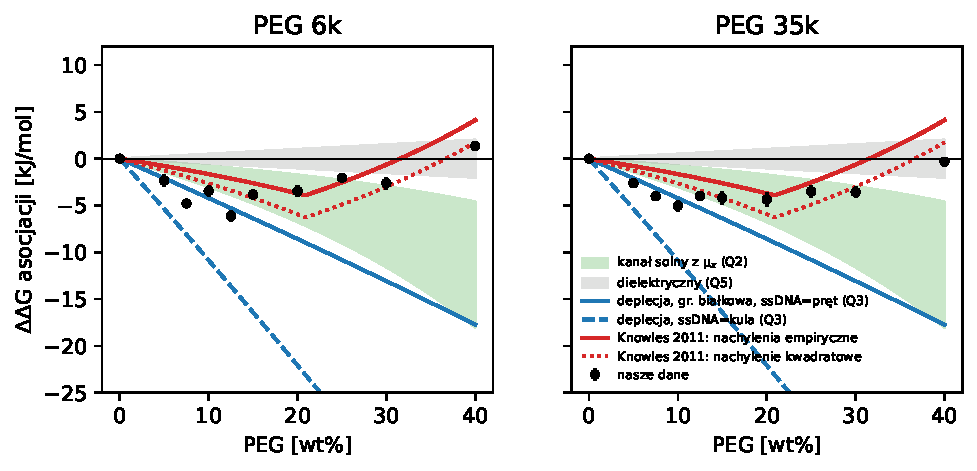
\includegraphics[width=0.98\linewidth]{lit_budget.pdf}
\caption{Nasze $\dG$ (punkty) vs człony wzięte wprost z literatury, bez dopasowania: nachylenia empiryczne Knowlesa (z odwróceniem przy 6 monomolal), deplecja w granicy białkowej (Q3), kanał solny z $\mu_x$ (Q2, NaCl i Na$_2$HPO$_4$ jako zakres) i pasmo dielektryczne (Q5). Skrypt: \texttt{lit\_budget.py}.}
\label{fig:budget}
\end{figure}

\section{Q1: bezpośrednie dowody oddziaływań EG/PEG z zasadami i ssDNA}

\textbf{Co wiadomo.}
\begin{itemize}
\item \emph{Rozpuszczalności/energie przeniesienia.} Kluczowe dane dla glikoli (Herskovits \& Harrington 1972 \cit{b:hersk72}) są niedostępne (brak abstraktu, paywall). Jedyna liczba z pełnego tekstu: adenina w 0.6 M adonitolu, $\log(S/S_0)=0.076$ przy 25.5~°C, czyli około $-0.17$~kcal\,mol$^{-1}$M$^{-1}$ \cit{b:tso63}\PT. Autorzy uznają poliol za „ineffective”.
\item \emph{Rachunek rzędu wielkości} (notatki Q1): nasza m-wartość EG wymaga tylko około $-0.02$ do $-0.04$~kcal\,mol$^{-1}$molal$^{-1}$ na zasadę (zmiana rozpuszczalności około 1\% na molal). Obraz Knowlesa nie wymaga więc silnego wiązania, ale też trudno go potwierdzić pomiarem rozpuszczalności.
\item \emph{NMR.} G-kwadrupleks, 25~°C, 100 mM KCl, 20~wt\% EG lub PEG 8000: \textbf{brak NOE} glikol--DNA; przesunięcia rdzenia $\le0.03$~ppm (EG), eksponowany T20 H6 do $+0.52$~ppm (PEG 8000) \cit{b:traj}\PT. Kontakty CH--$\pi$ pokazano tylko dla TEG przyłączonego kowalencyjnie, który dupleksu nie stabilizuje ($-6.6$ vs $-5.1$/$-5.9$~kcal/mol) \cit{b:tateishi}\PT. Wiązanie PEG 600 z G4 ($K_B=0.41$~M, około $-0.5$~kcal/mol na cząsteczkę) jest wnioskowane z modelu, nie zmierzone \cit{b:buscaglia}\PT.
\item \emph{MD.} EG lokalnie około 2× wzbogacony przy dupleksie B, głównie przy fosforanach (GAFF, 0.1 M NaCl) \cit{b:jaiswal}\PT. To kłóci się z VPO, gdzie grupy glikolowe są silnie wykluczane z HPO$_4^{2-}$ \cit{b:kn15}. Brak MD ssDNA i brak całek Kirkwooda--Buffa ss vs ds.
\item \emph{Grupa Recorda po 2011.} $\alpha$ PEG z grupami białkowymi: aromatyczny C $\alpha_I=-0.765$, końce $\alpha_{2E}=-0.364$~cal\,mol$^{-1}$molal$^{-1}$Å$^{-2}$; nukleozasady „are in progress” \cit{b:kn15}\PT. EG nie zachowuje się jak „dwa końce PEG” (m dla lacDBD 2× mniejsze). Reanaliza danych DNA: $\chi_\infty=0.6\pm0.06$; zależność od rozmiaru DNA „is unknown” \cit{b:shkel}\PT. W latach 2016--2026 brak publikacji o $\alpha$ glikol--zasada (lista prac Recorda w EPMC). Jako szablon metody: mocznik--grupy funkcyjne kwasów nukleinowych \cit{b:guinn}\PT.
\item \emph{Co komplikuje obraz.} Szkoła aktywności wody dostaje różne „liczby wody” dla różnych kosolutów (15 H$_2$O/bp PEG vs 4.7 glicerol; trzy osobne proste u Ghosh 2020) \cit{b:nakano04,b:ghosh20}\PT, co samo wskazuje na oddziaływania specyficzne. Osłabienie stackingu ssDNA daje tę samą sygnaturę termodynamiczną co solwatacja zasad.
\end{itemize}
\textbf{Co możemy policzyć.} Po zdobyciu Herskovits 1972: $\mu_{23}$ zasad w EG, podział przez ASA, przemnożenie przez $\Delta$ASA naszego 13-meru: przewidywanie m-wartości EG \emph{bez} danych DNA. Z $\alpha$ PEG--aromat (białkowe) półilościowe przewidywanie dla PEG 200.
\textbf{Czego nie ma.} NMR (HSQC/STD) ssDNA lub nukleozydów z wolnym EG/PEG; $\alpha$ glikol--zasada; $\chi$(rozmiar DNA); MD ss vs ds z KB.

\section{Q2: termodynamika PEG--sól i znak $\mu_x$}

\textbf{Co wiadomo} (konwencja: $\mu_x=(\partial\mu_\text{sól}/\partial m_\text{EO})_{m_s}$, cal\,mol$^{-1}$ na molal EO; $>0$ to wykluczenie soli).
\begin{itemize}
\item VPO, 25~°C, KCl: $+37.8\pm1$ (PEG 1000), $+32.4\pm1$ (PEG 2000); poliole $\approx0$ \cit{b:kn11}\PT (SI Tab. S3).
\item VPO, $<0.6$~m, rozkład na jony (grupa wewnętrzna EO): Na$^+$ $+4.66\pm2$, K$^+$ $+3.22\pm3.4$, Cl$^-$ $+37.6\pm2.4$, HPO$_4^{2-}$ $+234\pm5.5$; stąd NaCl $+42\pm3$, Na$_2$HPO$_4$ $+243\pm7$ \cit{b:kn15}\PT (tabelę odczytano niezależnie w dwóch przeszukiwaniach, wartości zgodne). H$_2$PO$_4^-$ nie mierzono.
\item Dyfuzja wieloskładnikowa, PEG 20k + NaCl: 2.4 H$_2$O na EO, czyli $\mu_x\approx+47$--50 \cit{b:annun24}\PT; siarczan około 3× więcej \cit{b:cruz}\PT.
\item Jedyny ujemny znak: aniony chaotropowe (NaClO$_4$ w PEG 4000, około $-60$ do $-65$) \cit{b:morales20}\PT. Salting-in przez SCN$^-$ wynika z wiązania \emph{anionu} \cit{b:mcafee15}\ABS.
\item Wiązanie kationów (nanopory, granice faz, rozpuszczalniki niewodne, DOSY): ocenione osobno w sekcji~\ref{sec:q8}.
\end{itemize}
\textbf{Co możemy policzyć (policzone, \texttt{q2\_mux\_estimate.py}).} Najlepszy szacunek: $\mu_x\approx+42\pm5$ (NaCl jako proxy) do około $+240$ (Na$_2$HPO$_4$). Wtedy $\partial\ln K/\partial m_\text{EO}\approx+0.12$ do $+0.48$ (stabilizacja) przy SK~$=3.5$. Dla PEG 35k: $\LsaltLofive$ do $\LsaltHifive$~kJ/mol przy 5\% i $\LsaltLofourzero$ do $\LsaltHifourzero$ przy 40\% (liniowo, górna wartość na pewno przeszacowana). Kanał solny ma więc przeciwny znak do mechanizmu Bielec 2022 i działa \emph{na korzyść} stabilizacji.
\textbf{Czego nie ma.} $\mu_x$ dla PEG + fosforan sodu w rozcieńczeniu; pełny tekst Morales 2009 (NaCl w PEG 4000, ISE); parametry krzyżowe z ATPS PEG--fosforan przy niskiej soli. Rozstrzyga \textbf{VPO w naszym buforze} ($\Delta$Osm = Osm(NaPi+PEG) $-$ Osm(NaPi) $-$ Osm(PEG), 0.1--0.3 m NaPi, PEG 1000 i EG, kontrola NaCl; oczekiwany sygnał 36--205 mOsm).

\section{Q3: deplecja w reżimie półrozcieńczonym}

\textbf{Wzory} (szczegóły i numery równań w \texttt{notes/Q3\_depletion.md}):
\begin{itemize}
\item Granica białkowa, kula (Hanke, Eisenriegler, Dietrich 1999, Eq.~1.5, 1.8, 2.54) \cit{b:hanke}\PT:
$\displaystyle \frac{\mu_\text{sph}}{kT}=A_{3,3}\,n_pR_x^{1/\nu}R^{3-1/\nu},\quad A_{3,3}=9.82$; pręt: $\displaystyle\frac{\mu_\text{cyl}}{kT\,L}=A_{2,3}\,n_pR_x^{1/\nu}r^{2-1/\nu},\quad A_{2,3}=1.23$. Ponieważ $n_pR_x^{1/\nu}\propto c$, $\mu$ jest \textbf{liniowe w stężeniu monomerów i niezależne od M}.
\item Półrozcieńczony (Odijk 1996, Eq.~5) \cit{b:odijk96}\PT: $w/kT=(a/\xi)^{4/3}\propto c$. Wykładnik wynosi $3-1/\nu\approx4/3$ względem rozmiaru cząstki; ani $1/\nu$, ani 5/3.
\item Granica koloidalna: $\mu=\Pi V+\gamma A$, $\Pi\propto c^{2.31}$, $\gamma\approx\tfrac32\Pi\xi\propto c^{1.54}$ \cit{b:louis}\PT; grubość warstwy $\delta=1.07R_g(1+3.95\phi^{1.54})^{-1/2}$ (L\&T Eq.~4.21) \cit{b:lt}\PT; $\Pi$ z równania stanu Cohena i in. \cit{b:cohen}\PT, którego człon półrozcieńczony nie zależy od M.
\end{itemize}
\textbf{Policzone} (\texttt{q3\_depletion\_exponents.py}, dsDNA = pręt $r=1$~nm, $L=4.4$~nm; ssDNA = pręt $r=0.5$, $L=8$ albo kula $R=1.5$~nm): granica białkowa daje $\dG_\text{dep}=\LdepRodfive$ do $\LdepSphfive$~kJ/mol przy 5\% i $\LdepRodfourzero$ do $\LdepSphfourzero$ przy 40\%. Efektywny wykładnik na skali monomolalnej $p\approx0.83$ (poniżej 1 tylko przez nieliniowość $x\propto w/(1-w)$). Modele GFVT i koloidalne dają $p=0.77$--1.53. \textbf{Żaden wariant nie daje nasycenia ani odwrócenia.}
\textbf{Wnioski dla nas.} (i) Niezależność od M na skali monomeru wskazuje na granicę białkową. (ii) Liniowa deplecja i liniowe preferencyjne oddziaływania są nierozróżnialne po samej zależności od $x$, rozróżnia je tylko znak i geometria. (iii) Nasze wczesne nasycenie przy około 5~wt\% nie wynika z żadnej z tych teorii. Zosel i in. \cit{b:zosel}\PT dla IDP musieli użyć przenikalnego „segmentu” 0.4~nm zamiast pełnej kuli, co sugeruje, że realna deplecja ssDNA jest bliżej wariantu „pręt”.
\textbf{Czego nie ma.} Ścisłych wyników dla obiektów o rozmiarze około $\xi$ (u nas $\xi=0.8$--2.3~nm); amplitudy SRE dla krótkich prętów w półrozcieńczonym; teorii dla przenikalnego, naładowanego ssDNA. Pracy Eisenriegler 2000 (półrozcieńczony, małe cząstki) \cit{b:eis00} nie udało się przeczytać.

\section{Q4: dupleksy i spinki w EG/PEG; prace cytujące Bielec 2022}

\textbf{Co wiadomo.}
\begin{itemize}
\item \emph{Sól ustala znak.} Markarian \& Schlenoff \cit{b:markarian}\PT: 15--35-mery, PEG 3k 1--30\%, a(Na$^+$) $<0.05$: $K$ rośnie z PEG; $\ge0.05$: maleje; PEG \emph{obniża} [NaCl] potrzebne do parowania. Nakano 2004 \cit{b:nakano04}\PT (1 M NaCl): żaden PEG nie stabilizuje 8-meru; PEG 8000 10--20\% destabilizuje o +0.5 do +1.2~kcal/mol. Karimata 2007 \cit{b:karimata07}\ABS: PEG 8000 stabilizuje przy niskim NaCl, destabilizuje przy wysokim; „PEG buffers sodium ion binding”.
\item \emph{Odwrócenie i skala monomeru.} Jedyną pracą z jawną niezależnością od M na skali monomolalnej i odwróceniem przy około 6 monomolal jest Knowles 2011 \cit{b:kn11}\PT. Odwrócenie dotyczy dupleksu, nie spinki.
\item \emph{Duże efekty przy małych stężeniach w pomiarach fluorescencyjnych.} Spinka DNA, smFRET, 10\% w/w: $\dG=-5.1$ (PEG 400) i $-7.2$~kJ/mol (PEG 8000) \cit{b:baltierra}\PT. Motyw RNA: PEG 8000 4\% daje K$\times$6.3 \cit{b:dupuis}\PT. Pasuje to do naszej szybkiej stabilizacji, ale dotyczy procesów jednocząsteczkowych.
\item \emph{Testy mechanizmu Na$^+$.} Destabilizacja przez 40\% PEG 200 jest \emph{większa} przy 1 M (+4.4) niż przy 0.1 M NaCl (+3.0~kcal/mol) \cit{b:nakano04}\PT; Ghosh 2020: niezależna od soli \cit{b:ghosh20}\PT. Prosta sekwestracja kationu nie zmienia nachylenia $d\ln K/d\ln[\text{Na}^+]$, a kilka prac raportuje spadek $-\Delta n_{\text{Na}^+}$ w PEG \cit{b:karimata07,b:spink99}\ABS.
\item \emph{Prace cytujące Bielec 2022} (Crossref/OpenAlex 11 rekordów, 9 unikalnych): 4 to autocytowania lub IChF (Kowalski 2022, Kowalski 2025, Kwapiszewska 2024, Karpińska 2022); Silva \& Weber 2026 przyjmuje mechanizm bez testu \cit{b:silva}\PT; pozostałe cytują pobocznie. Żadna praca nie testuje mechanizmu ani mu jawnie nie przeczy.
\item \emph{Napięcie wewnętrzne.} Bielec 2022 pisze, że poniżej kilku wt\% zmiana $K$ jest „nearly negligible”, a nasze obecne dane dają $K\times5$--11 przy kilku wt\% długiego PEG. Trzeba to wyjaśnić w manuskrypcie.
\end{itemize}
\textbf{Co możemy policzyć.} Porównanie liczbowe z Knowlesem (rys.~\ref{fig:budget}): w przybliżeniu zgodne przy 20--40\%, dla długich PEG 2--3× szybszy początek. Zgodność ilościowa dla EG i PEG 200 przy 40\% (pkt 1 na pierwszej stronie).
\textbf{Czego nie ma.} Pełnego tekstu Karimata 2007 (próg NaCl zmiany znaku); pomiarów całej krzywej 0--40\% dla wielu M przy niskiej soli poza Knowlesem i nami; dwucząsteczkowej hybrydyzacji w PEG mierzonej smFRET/FCS (poza naszą grupą).

\section{Q5: stała dielektryczna i aktywność wody}
\begin{itemize}
\item $\varepsilon$ w 25~°C: EG 40 wt\% $\approx67.5$ (przeskalowane z serii z około 20~°C \cit{b:kaiser}\PT); PEG 400 40 wt\% $\approx58$--61 (1--2 MHz; tabela $\varepsilon$ mieszanin woda--PEG 400 w pracy o acetaminofenie) \cit{b:yurquina}\PT. Dla PEG $\ge1000$ brak pomiarów w dostępie. Wartość 56.74 z SI Bielec 2022 pochodzi z obliczenia liniowego mieszania dla 40\% v/v \cit{b:panraksa}\PT.
\item \emph{Policzone} (\texttt{q5\_dielectric\_PB.py}, nieliniowy PB, cylindry, skok ssDNA kalibrowany na nasze nachylenie solne 3.49): $|\dG_\text{diel}|\lesssim2$~kJ/mol, znak zależy od promienia ssDNA. Obserwujemy +14.7 (EG) i +9.6~kJ/mol (PEG 400). Przewidywanie testowalne: nachylenie solne spada do około 3.2--3.3 w 40\% EG.
\item EG jest wykluczany z DNA tylko w około 5\% \cit{b:stanley}\PT; EG akumuluje się na ssDNA \cit{b:nordstrom}\ABS; kolejność stabilności w kosolwentach nie śledzi $\varepsilon$ \cit{b:hickey}\ABS.
\item \emph{Aktywność wody} (\texttt{q5\_water\_activity.py}): pozorne $n_\text{app}$ dla EG = 2.4--3.2 H$_2$O/bp, zgodne z literaturą dla EG (1.8--4.1 \cit{b:rozners}\PT, około 4 \cit{b:spink99}\ABS). Dla PEG $\ge3$k samo a$_w$ przewiduje +11--12~kJ/mol, a obserwujemy około 0. Wartości a$_w$ z Nakano 2004 zmierzono w 1 M NaCl i dla PEG są około 3× większe niż wynika z równania stanu, więc nie przenoszą się na nasz bufor.
\item \emph{Rozdzielenie.} Z jednym kosolutem a$_w$ i oddziaływania preferencyjne są nierozdzielne (to ta sama wielkość, Parsegian, Rand, Rau 2000 \cit{b:parsegian}\PT). Szereg EG $\to$ PEG 35k działa jak zestaw kosolutów w duchu Knowlesa.
\end{itemize}
\textbf{Czego nie ma.} $d\ln K/d(1/\varepsilon)$ przy stałej soli dla krótkich dupleksów; $\varepsilon$ dla PEG $\ge1000$; a$_w$ dla PEG/EG w niskiej soli przy 25~°C.

\section{Q6: fotofizyka i stacking Atto488/Atto647N}
\begin{itemize}
\item Stacking barwników na tym samym końcu: $K=(3.5\pm1.9)\cdot10^9$ vs $(1.1\pm0.5)\cdot10^9$~M$^{-1}$ (barwniki na przeciwnych końcach), około $-2.75$~kJ/mol; różnica około 1.2$\sigma$; jasność Atto488 rośnie o 22\% po hybrydyzacji \cit{b:bielec20}\PT.
\item Atto647N: ładunek $+0.61$, logD $+1.96$ \cit{b:zanetti}\PT; MIF 1361, logD do 3.82; Atto488 MIF 0.007 \cit{b:hughes}\PT. Cyjaniny na końcach dupleksu stabilizują go o około 1.2~kcal/mol \cit{b:moreira}\ABS i stackują jak dodatkowa para \cit{b:iqbal}\PT.
\item Atto488 i Atto647N nie izomeryzują jak cyjaniny, więc efekt lepkości na $\Phi$ jest mało prawdopodobny. Zmiana $n$ z 1.333 na około 1.39 podnosi $k_r$ o około 9\%, $\Phi$ Atto488 o $\le2$\% \cit{b:toptygin}. Badań tych barwników w PEG/EG nie znaleziono.
\end{itemize}
\textbf{Ryzyko dla nas.} Jeśli crowder osłabia stacking barwników, do $\dG$ wchodzi do +2.7~kJ/mol, czyli przy długich PEG tyle co cały efekt. Glikole i glikoetery osłabiają stacking zasad \cit{b:feng}\PT. Akceptor jest nominalny, a adsorpcja kationowego, hydrofobowego Atto647N może zależeć od crowdera.
\textbf{Kontrole:} $K$ pary z jednym znacznikiem w EG 40\%, PEG 400 40\%, PEG 35k 20\% równolegle z parą FRET; FCS w kanale czerwonym (rzeczywiste $C_B$); potwierdzić w SI, że $\alpha$ i $\gamma$ mierzono w każdym roztworze.

\section{Q7: Henning-Knechtel et al., NAR 54, gkag752 (2026)}
Praca istnieje (Crossref; pełny tekst PMC13425243 i preprint bioRxiv) \cit{b:hk26}\PT. MD: GROMACS, OL3 + CUFIX, Na$^+$/Cl$^-$ Joung--Cheatham, TIP4P, PEG 6000 GAFF/RESP (walidacja tylko $R_g$ i gęstości), 150 mM NaCl, 165 g/L (około 14~wt\%), 310~K, 2$\times$2~\textmu s, spinka TAR 52 nt. Na$^+$ w promieniu 6~Å: 41 jonów (około 80\% neutralizacji) zarówno bez crowdera, jak i w PEG; „PEG exhibits limited association with Na$^+$”. Białka obniżają kondensację (60\% w abstrakcie, 40\% w dyskusji: niespójność). \textbf{Znaczenie:} jakościowo przeciw $\kappa\approx0.5$~M$^{-1}$ (wiązałoby około 65\% Na$^+$), ale pole siłowe Na$^+$--eter nie jest walidowane, liczba jonów skondensowanych jest mało czuła na aktywność objętościową, a warunki są inne niż nasze. Nie cytuje Bielec 2022.

\section{Q8: Ocena argumentów za wiązaniem Na$^+$/K$^+$ przez PEG}\label{sec:q8}
\textbf{Wspólna oś.} Wszystkie liczby wyrażam jako przyczynek kationu do $\mu_x$ w konwencji Knowles 2015: $\mu_+$ w cal\,mol$^{-1}$(molal EO)$^{-1}$, $>0$ to wykluczenie, $<0$ akumulacja. Dla słabego wiązania 1:1 ze stałą $\kappa$ na EO $\mu_+\approx-RT\kappa$ (granica liniowa; $\kappa$ w M$^{-1}$ traktuję jak molal$^{-1}$, błąd $<10$\%). Dla soli podaję $\mu_x$ całej soli (oznaczone „sól”). Przeliczenia: \texttt{q8\_cation\_binding.py} (wyniki w \texttt{.json}). Punkt odniesienia: 18-korona-6 w wodzie, $\log K=0.8$ (Na$^+$) i 2.03 (K$^+$) \cit{b:canj86}\textsuperscript{[snippet]}. To makrocykl ze wstępnie zorganizowanymi 6 tlenami; otwarty łańcuch wiąże słabiej (efekt makrocykliczny, wiedza podręcznikowa, bez weryfikacji liczbowej). Górne oszacowanie na EO, $K/6$: $\kappa\le1.05$~M$^{-1}$ ($\mu_+\ge-620$~cal) dla Na$^+$ i $\le18$~M$^{-1}$ ($\ge-10\,600$) dla K$^+$.

\scriptsize
\setlength{\tabcolsep}{2pt}
\begin{longtable}{>{\raggedright}p{2.1cm}>{\raggedright}p{1.55cm}>{\raggedright}p{1.5cm}>{\raggedright}p{3.4cm}>{\raggedright}p{2.9cm}>{\raggedright}p{1.65cm}>{\raggedright}p{1.45cm}>{\raggedright\arraybackslash}p{1.7cm}}
\toprule
praca & środowisko & kation, sól & zmierzone wprost / wywnioskowane & alternatywy; czy wykluczone & $\mu_+$ [cal] & przenośność & werdykt\\
\midrule\endhead
Knowles 2015 VPO \cit{b:kn15}\PT & woda rozc., $<0.6$~m & Na$^+$, K$^+$, Cl$^-$, HPO$_4^{2-}$ & wprost: osmolalność mieszanin; podział na jony z dopasowania wielu soli (ekstratermodynamiczny) & podział na jony zależy od konwencji; suma dla soli nie & Na$^+$ $+4.7\pm2$, K$^+$ $+3.2\pm3.4$; NaCl $+42$ (sól) & dobra (mała sól, mały PEG) & \textbf{mocny dowód w wodzie objętościowej} (brak akumulacji)\\
Knowles 2011 VPO \cit{b:kn11}\PT & woda rozc. & K$^+$, KCl & wprost: osmolalność & — & KCl $+32$ do $+38$ (sól) & dobra & \textbf{mocny dowód} (sól wykluczana)\\
Annunziata, dyfuzja \cit{b:annun24}\PT & woda rozc., PEG 20k 0.5\% & Na$^+$, NaCl 0.1--1 m & wprost: współczynniki dyfuzji krzyżowej + izopiestyka; wywnioskowane: 2.4 H$_2$O/EO & — & NaCl $+47$ do $+50$ (sól) & dobra & \textbf{mocny dowód}, niezależny od VPO\\
Bielec 2022, ISE \cit{b:bielec22}\PT & woda, 40 wt\% EG, glicerol & Na$^+$, 0.01--100 mM & wprost: kalibracje elektrody; przesunięcie około 6 mV, takie samo bez Na$^+$ & potencjał dyfuzyjny / rozpuszczalnik tłumaczy całość; PEG brudzi membranę (brak danych) & EG: $\ge-23$ (granica, zgodne z 0) & dobra dla EG, brak dla PEG & \textbf{sprzeczne} z wiązaniem (EG)\\
nasze DOSY, EG i PEG 200 & woda, 10--40 wt\% & Na$^+$, 35 mM & wprost: $D_\text{Na}$ i $D_\text{cr}$; stosunek spowolnień $0.999\pm0.023$; wywnioskowane: $\beta n$ & — & EG $+20\pm90$; PEG 200 $-5\pm17$ & nasze warunki & \textbf{mocny dowód} (brak wiązania)\\
nasze DOSY, PEG $\ge$1000 & woda, 10--40 wt\% & Na$^+$, 35 mM & wprost: nadmiarowe spowolnienie Na$^+$; wywnioskowane: $\kappa$ z modelu dwustanowego + poprawki lepkościowej & przeszkody i nanolepkość (rozrzut 3× od poprawki); kontakty przejściowe bez zmiany aktywności: niewykluczone & $-33$ do $-100$ & nasze warunki & \textbf{zgodne, ale niejednoznaczne}\\
Bielec 2022, $\kappa=0.49$ \cit{b:bielec22}\PT & woda, 40 wt\% & Na$^+$, 10--125 mM & wprost: $K(c_\text{Na})$; wywnioskowane: $\kappa$ z poziomego przesunięcia (zakłada A) & B (przy potęgowym $F$ identyczne), C (nachylenie się zmienia): niewykluczone; argument kołowy & $-290$ & nasze warunki & \textbf{słabe lub kołowe}\\
Markarian \& Schlenoff 2010 \cit{b:markarian}\PT & woda, PEG 3k 0--30 wt\% & Na$^+$, 2--225 mM & wprost: $K$ vs a$_\text{Na}$ (a$_\text{Na}$ z VPO przy założeniu braku wiązania); PEG \emph{obniża} [NaCl] potrzebne do parowania & autorzy: mniej jonów wiązanych przez nici (C) & nie\-prze\-li\-czal\-ne & dobra & \textbf{sprzeczne} z wiązaniem przez PEG\\
Karimata 2007 \cit{b:karimata07}\ABS & woda & Na$^+$, różne NaCl & wprost: $T_m$ vs [NaCl]; wywnioskowane: spadek $-\Delta n_\text{Na}$, „PEG buffers sodium ion binding” & prosta sekwestracja nie zmienia nachylenia; $\varepsilon$, C: niewykluczone & nie\-prze\-li\-czal\-ne & dobra & \textbf{zgodne, ale niejednoznaczne}\\
Spink \& Chaires 1999 \cit{b:spink99}\ABS & woda, EG & Na$^+$ & wprost: $T_m$; wywnioskowane: wiązanie przeciwjonów \emph{przez DNA} nieco maleje ze spadkiem a$_w$ & dotyczy DNA--jon, nie PEG--jon & nie\-prze\-li\-czal\-ne & średnia & \textbf{zgodne, ale niejednoznaczne}\\
Henning-Knechtel 2026, MD \cit{b:hk26}\PT & woda, 14 wt\% PEG 6000 & Na$^+$, 150 mM & symulacja: „limited association” PEG--Na$^+$; liczba Na$^+$ przy RNA bez zmian & pole siłowe Na$^+$--eter niewalidowane & nie\-prze\-li\-czal\-ne (Fig. S17 nieczytana) & średnia & \textbf{zgodne, ale niejednoznaczne} (przeciw dużemu $\kappa$)\\
Silva \& Weber 2026 \cit{b:silva}\PT & model mezo\-sko\-po\-wy & Na$^+$ 122 mM & nic; przyjmuje kompleksowanie za Bielec 2022 & — & — & — & \textbf{słabe lub kołowe}\\
Rodrigues 2008 \cit{b:rodrigues}\PT & por $\alpha$-HL & K$^+$, 1--4 M & wprost: energia PEG--por 0.03--0.27~kT na monomer; wywnioskowane: kompleksowanie K$^+$ (hipoteza za Okadą) & wysalanie PEG do poru: niewydzielone & $-18$ do $-40$ (założenie: cała energia z wiązania K$^+$, Langmuir liniowy) & słaba (por, 1--4 M) & \textbf{prawdziwe, ale inne środowisko}\\
Reiner 2010 \cit{b:reiner}\ABS & por (teoria + dane) & K$^+$, wysoka sól & wywnioskowane: $\Delta G$ kompleksu K$^+$--PEG w porze $\approx-1.9$~kT & stechiometria nieznana & nie\-prze\-li\-czal\-ne & słaba & \textbf{prawdziwe, ale inne środowisko}\\
Breton 2013 \cit{b:breton}\ABS & por & Li$^+$--Cs$^+$, wysoka sól & wprost: PEG zachowuje się jak naładowany dla wszystkich kationów poza Li$^+$ & specyficzność kationowa przemawia za kationem; liczby za paywallem & nie\-prze\-li\-czal\-ne & słaba & \textbf{prawdziwe, ale inne środowisko}\\
Ohki, Harada, Okada 2007 \cit{b:ohki}\ABS & granica woda/\-nitro\-benzen; około 33\% PEG 200 & K$^+$ & wprost: XAFS kompleksu K$^+$ w stężonym PEG 200; transfer jonów przez granicę faz & autorzy: przy niskim PEG kompleks „at the interface rather than in bulk” & nie\-prze\-li\-czal\-ne & słaba & \textbf{prawdziwe, ale inne środowisko}\\
Okada 1991 \cit{b:okada91}\ABS & faza żywicy jono\-wymien\-nej & metale alkaliczne & selektywność kationów & brak wody objętościowej & nie\-prze\-li\-czal\-ne & brak & \textbf{prawdziwe, ale inne środowisko}\\
Hakem 2004, SANS \cit{b:hakem}\ABS & roz\-pusz\-czal\-ni\-ki o różnej $\varepsilon$ & jony jedno\-war\-to\-ścio\-we & wiązanie w rozpuszczalnikach o niskiej $\varepsilon$; przy wysokiej $\varepsilon$ i wiązaniach H „PEO effectively remains a neutral polymer” & — & nie\-prze\-li\-czal\-ne ($\approx0$ dla wody, jakościowo) & średnia & \textbf{prawdziwe, ale inne środowisko}; dla wody przeciw\\
Elektrolity PEO \cit{b:fenton}\textsuperscript{[META]} & ciało stałe, stop & Li$^+$, Na$^+$, K$^+$ & krystaliczne kompleksy PEO--sól (koordynacja przez tlen eterowy) & — & nie\-prze\-li\-czal\-ne & brak (bez wody) & \textbf{prawdziwe, ale inne środowisko}\\
\bottomrule
\end{longtable}
\normalsize

\begin{figure}[h]
\centering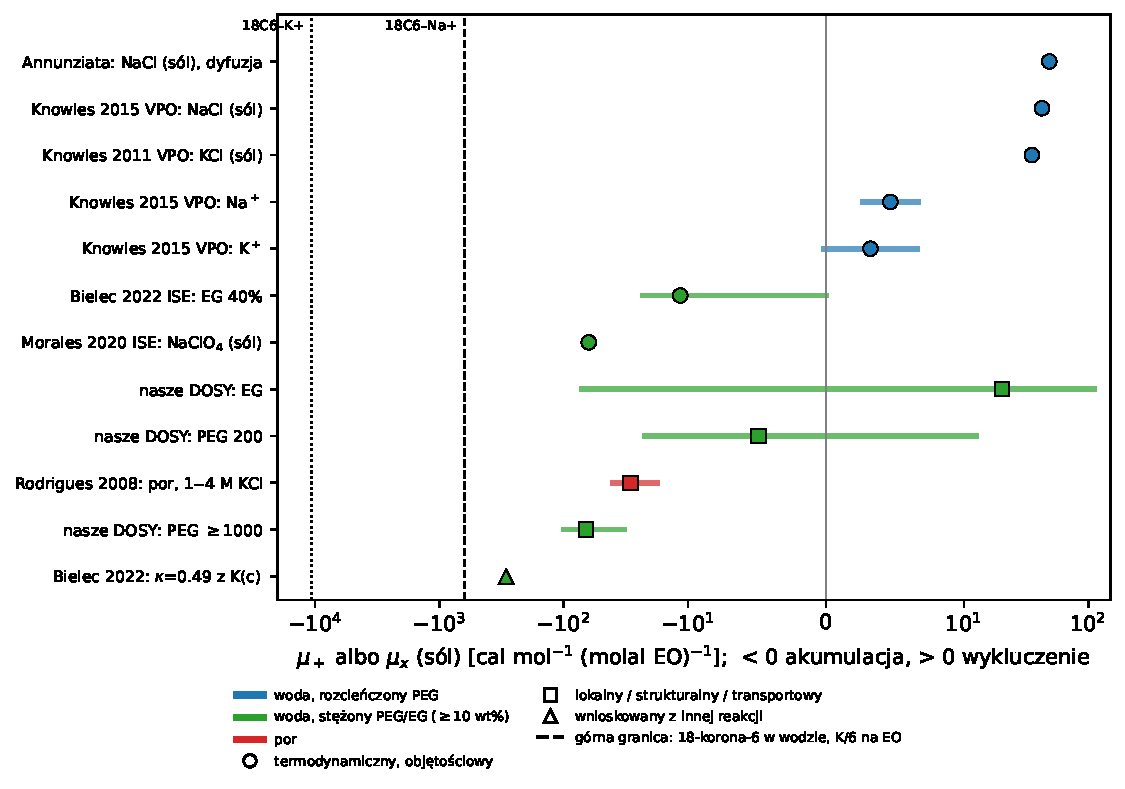
\includegraphics[width=0.9\linewidth]{q8_cation_binding.pdf}
\caption{Wszystkie przeliczalne liczby na wspólnej osi (skala symlog, liniowa w $\pm10$). Kolor: środowisko; kształt: typ pomiaru. Linie pionowe: 18-korona-6 w wodzie podzielona przez 6 EO (górne oszacowanie dla otwartego łańcucha). Pozycje nieprzeliczalne są w tabeli. Skrypt \texttt{q8\_cation\_binding.py}.}
\label{fig:q8}
\end{figure}

\textbf{Trend.} Hipoteza „im bardziej pośrednio i im mniej wody, tym silniejsze wiązanie” się potwierdza. Termodynamika objętościowa w rozcieńczonej wodzie daje dla kationu $0$ do $+5$~cal, a dla soli $+32$ do $+50$. Transport w stężonym PEG (DOSY) daje $-33$ do $-100$. Wnioskowanie z $K$ hybrydyzacji daje $-290$. Poza wodą objętościową (pory, granica faz, żywice, ciało stałe, rozpuszczalniki o niskiej $\varepsilon$) wiązanie jest wyraźne, ale nieprzeliczalne. Jedyny wyjątek od monotoniczności to nanopor: przeliczona energia na monomer jest mała ($-18$ do $-40$), a efekt „naładowanego PEG” bierze się z sumowania po kilkudziesięciu monomerach przy 1--4~M soli. Wartość z Bielec 2022 to połowa górnej granicy z 18-korony-6 (na EO), czyli otwarty łańcuch musiałby wiązać Na$^+$ prawie jak makrocykl.

\textbf{Synteza.}
\begin{itemize}[leftmargin=*]
\item \emph{Co wiemy.} W rozcieńczonym roztworze wodnym ($<0.6$~m soli, mały PEG) \textbf{nie ma akumulacji netto} soli przy PEG; sól jest wykluczana ($\mu_x>0$, trzy metody, zgodność około 15\%). Pewność znaku jest wysoka. Wartość dla samego Na$^+$ ($+4.7\pm2$) ma średnią pewność, bo podział na jony jest ekstratermodynamiczny.
\item \emph{Pogodzenie z koordynacją.} $\Gamma_\text{Na}=\Gamma_\text{koord}-\Gamma_\text{wypchn}$. DOSY widzi $\Gamma_\text{koord}$ (czas spędzony przy łańcuchu spowalnia jon), ale nie widzi wykluczenia (wypchnięty jon porusza się swobodnie). VPO, ISE i dyfuzja wieloskładnikowa widzą tylko sumę, a od sumy zależy $K$. Nanopory i XAFS widzą koordynację lokalną, wzmocnioną zamknięciem, stężeniem lub dużą solą. Model: wykluczenie z 2.4 H$_2$O/EO daje każdemu jonowi $+RT\cdot2.4/55.5=+26$~cal; przy zmierzonym $+4.7$ zostaje miejsce na koordynację $\kappa\approx0.035$~M$^{-1}$. Dolne $\kappa$ z DOSY (0.055) wymaga wykluczenia z około 3.5 H$_2$O/EO, górne (0.17) z około 9.8, czyli 4× więcej niż zmierzone. Dolne DOSY da się więc pogodzić z VPO, górnego i $\kappa=0.49$ nie.
\item \emph{Największa luka.} Brak termodynamiki (aktywności soli) przy 20--40~wt\% PEG i przy naszej soli: VPO Knowlesa kończy się na $<0.6$~m, a jedyny pomiar ISE dla NaCl w PEG 4000 do 25~wt\% (Morales 2009) znamy tylko z metadanych. Brak też pomiaru specyficznego dla Na$^+$ w objętości (np. relaksacja lub przesunięcie $^{23}$Na NMR w PEG $\ge$1000 vs EG).
\end{itemize}

\textbf{Steelman.} Najmocniejszy argument za akumulacją Na$^+$ w wodzie to nasze DOSY dla PEG $\ge$1000: pomiar w wodzie objętościowej, w naszych warunkach, z dodatnim nadmiarem spowolnienia przy każdej poprawce lepkościowej i z progiem długości łańcucha (EG i PEG 200: zero), czego oczekuje się po chelatowaniu wieloma tlenami. Chemicznie jest to wiarygodne, bo 18-korona-6 wiąże Na$^+$ w wodzie mierzalnie ($\log K=0.8$), a nanopory pokazują specyficzność kationową (Li$^+$ inaczej niż Na$^+$--Cs$^+$). Argument przegrywa jednak z bilansem: wielkość, którą widzi DNA, to aktywność netto, a ta jest dodatnia.

\section{Tabela liczb do użycia}
\small
\begin{longtable}{>{\raggedright}p{4.1cm}>{\raggedright}p{2.6cm}>{\raggedright}p{4.3cm}p{1.2cm}p{1.1cm}}
\toprule
wielkość & wartość & warunki & źródło & dostęp\\
\midrule\endhead
m/N EG--triEG, dupleks (topnienie) & $-0.340\pm0.01$ kcal/molal & 12 bp, 0.14 m K$^+$, 313 K & \cit{b:kn11} & PT\\
m/N PEG 200, dupleks & $-0.21\pm0.01$ & jw. & \cit{b:kn11} & PT\\
m/N plateau PEG $\ge2000$ & $+0.156\pm0.020$ (liniowo); $+0.25\pm0.05$ (kwadr.) & jw., do 5 monomolal & \cit{b:kn11} & PT\\
odwrócenie stabilizacji & centrum około 6 monomolal & PEG 2000--8000, dupleks & \cit{b:kn11} & PT\\
$\chi_\infty$ & $0.45\pm0.10$ / $0.6\pm0.06$ & 12-mery, 40 °C & \cit{b:kn11,b:shkel} & PT\\
$\alpha_I$, $\alpha_{2E}$ (aromat. C) & $-0.765$, $-0.364$ cal mol$^{-1}$molal$^{-1}$Å$^{-2}$ & związki modelowe białek, VPO 25 °C & \cit{b:kn15} & PT\\
$\beta_I$: Na$^+$, K$^+$, Cl$^-$, HPO$_4^{2-}$ & $+4.66$, $+3.22$, $+37.6$, $+234$ cal mol$^{-1}$molal$^{-1}$ & VPO $<0.6$ m, 25 °C & \cit{b:kn15} & PT\\
$\mu_x$ PEG--KCl & $+37.8$ (PEG 1000), $+32.4$ (PEG 2000) cal & VPO, 25 °C & \cit{b:kn11} & PT\\
$\mu_x$ PEG 20k--NaCl & około $+47$--50 cal (2.4 H$_2$O/EO) & dyfuzja, 25 °C & \cit{b:annun24} & PT\\
$\mu_x$ PEG 4000--NaClO$_4$ & około $-60$ do $-65$ cal & ISE, 298 K & \cit{b:morales20} & PT\\
$A_{3,3}$, $A_{2,3}$ & 9.82, 1.23 & SRE, dobry rozp. & \cit{b:hanke} & PT\\
$\alpha$ (EOS PEG) & $0.49\pm0.01$; $\bar V=0.825$ mL/g & woda, PEG & \cit{b:cohen} & PT\\
$\delta(\phi)$ & $1.07R_g(1+3.95\phi^{1.54})^{-1/2}$ & dobry rozp. & \cit{b:lt} & PT\\
$\varepsilon$ EG 40 wt\% / PEG 400 40 wt\% & około 67.5 / 58--61 & 25 °C (EG przeskalowane) & \cit{b:kaiser,b:yurquina} & PT\\
$\Delta n_w$ EG & 1.8--4.1 H$_2$O/bp & 6--12 bp, 0.3 M NaCl & \cit{b:rozners} & PT\\
$\Delta n_w$ PEG 200--8000 & $15.0\pm0.6$ H$_2$O/bp & 8-mer, 1 M NaCl & \cit{b:nakano04} & PT\\
wykluczenie EG z DNA & $0.05\pm0.01$ & macierze DNA, 20 °C & \cit{b:stanley} & PT\\
$\dG$ spinki, 10\% PEG 400 / 8000 & $-1.23\pm0.06$ / $-1.73\pm0.03$ kcal/mol & smFRET & \cit{b:baltierra} & PT\\
stacking Atto488/Atto647N (ten sam koniec) & $K$ około 3× (około $-2.75$ kJ/mol), 1.2$\sigma$ & 20 mM PB, 25 °C & \cit{b:bielec20} & PT\\
Atto647N: MIF, logD & 1361; 1.96--3.82 & lipidy egg-PC; pH 7.4 & \cit{b:hughes,b:zanetti} & PT\\
\bottomrule
\end{longtable}
\normalsize

\section{Luki w literaturze, czyli nasza potencjalna nowość}
\begin{enumerate}[leftmargin=*]
\item Pełna krzywa $K$(0--40~wt\%) dla 11 crowderów EG$\to$PEG 35k przy \emph{niskiej} soli (35 mM Na$^+$), 25~°C, dla hybrydyzacji dwucząsteczkowej; dotąd tylko Knowles (0.14 m K$^+$, 40~°C, do 8000/20000).
\item Wczesne nasycenie stabilizacji przy kilku wt\%: nieopisane i niewyjaśnione przez teorię deplecji ani przez obraz Knowlesa (o ile nie jest artefaktem barwnikowym).
\item DOSY Na$^+$ w szeregu homologicznym z progiem długości łańcucha (EG i PEG 200 bez wiązania). Nikt nie zestawił pomiaru dyfuzyjnego z $\mu_x$ z VPO; w połączeniu daje to rozkład $\mu_x$ na składowe kationowa i anionowa, czego brak w literaturze.
\item $\mu_x$ dla PEG + fosforan sodu w niskiej soli (VPO) i test przesunięcia maksimum $K(c_\text{Na})$ w poziomie lub pionie: brak w literaturze, rozstrzygają spór o mechanizm Na$^+$.
\item $\alpha$ glikol/PEG--zasada i $\chi$(rozmiar DNA): zapowiadane przez Recorda, nieopublikowane.
\item Wpływ crowderów na stacking barwników w parach FRET: brak danych.
\end{enumerate}

\section{Ograniczenia przeglądu}\label{sec:ogr}
\begin{itemize}
\item Pełnych tekstów nie mamy dla: Herskovits \& Harrington 1972, Karimata 2007, Morales 2009, Spink \& Chaires 1999, prac ATPS PEG--fosforan, Eisenriegler 2000, Breton 2013. Warto je zamówić przez bibliotekę IChF.
\item Werdykt sekcji~\ref{sec:q8} opiera się w kilku miejscach tylko na abstraktach lub metadanych: Morales 2009 (ISE, NaCl w PEG 4000; najbardziej bezpośredni brakujący pomiar aktywności), Karimata 2007 (próg NaCl, $-\Delta n_\text{Na}$), Breton 2013 (liczby skompleksowanych kationów w porze), Ohki 2007 (warunki XAFS), Hakem 2004 (rozpuszczalniki, parametry wiązania), Okada 1990/1991, Reiner 2010, Fenton 1973 (tylko metadane), Spink \& Chaires 1999. Stałe 18-korony-6 w wodzie (0.8 i 2.03) pochodzą z tabeli w Can. J. Chem. 1986 widzianej tylko jako fragment wyniku wyszukiwania (pełny tekst: 403); wartość dla Na$^+$ potwierdza drugi fragment (0.82, NMR). Fig.~S17 z Henning-Knechtel 2026 (liczba Na$^+$ przy PEG) nie była czytana. Dla tej sekcji wykonano jedno nowe wyszukiwanie (stałe eterów koronowych); pozostałe dane pochodzą z notatek Q2/Q4 i \texttt{salt\_shift/}.
\item Część pełnych tekstów z PMC czytano jako HTML z ekstrakcją przez model pomocniczy; kluczowa tabela $\beta$ z Knowles 2015 została odczytana niezależnie dwa razy z identycznym wynikiem.
\item Incydent techniczny: jedno z przeszukiwań wykonało \texttt{rm -f *.pdf} we wspólnym folderze \texttt{review\_2026-10/} na początku pracy. Drugie przeszukiwanie zgłosiło utratę dwóch plików, które pobrało ponownie do własnego podfolderu. Nie można wykluczyć utraty innego pliku z tego okna czasowego; notatki nie odwołują się do brakujących plików.
\end{itemize}

\section*{Bibliografia}
\small
\begin{enumerate}[label={[\arabic*]},ref={\arabic*},leftmargin=*,itemsep=0pt]
\item\label{b:kn11} Knowles D.B., LaCroix A.S., Deines N.F., Shkel I., Record M.T. Jr. Separation of preferential interaction and excluded volume effects on DNA duplex and hairpin stability. \emph{PNAS} 108, 12699 (2011). DOI 10.1073/pnas.1103382108. [CR; PT+SI]
\item\label{b:kn15} Knowles D.B., Shkel I.A., Phan N.M., et al., Record M.T. Jr. Chemical Interactions of Polyethylene Glycols (PEGs) and Glycerol with Protein Functional Groups: Applications to Effects of PEG and Glycerol on Protein Processes. \emph{Biochemistry} 54, 3528 (2015). DOI 10.1021/acs.biochem.5b00246. [CR; PT, PMC4464906]
\item\label{b:shkel} Shkel I.A., Knowles D.B., Record M.T. Jr. Separating chemical and excluded volume interactions of polyethylene glycols with native proteins: Comparison with PEG effects on DNA helix formation. \emph{Biopolymers} 103, 517 (2015). DOI 10.1002/bip.22662. [CR; PT]
\item\label{b:guinn} Guinn E.J., Schwinefus J.J., Cha H.K., et al. Quantifying Functional Group Interactions That Determine Urea Effects on Nucleic Acid Helix Formation. \emph{JACS} 135, 5828 (2013). DOI 10.1021/ja400965n. [CR; PT]
\item\label{b:hersk72} Herskovits T.T., Harrington J.P. Solution studies of the nucleic acid bases and related model compounds. Solubility in aqueous alcohol and glycol solutions. \emph{Biochemistry} 11, 4800 (1972). DOI 10.1021/bi00775a025. [CR; brak dostępu]
\item\label{b:tso63} Ts'o P.O.P., Melvin I.S., Olson A.C. Interaction and Association of Bases and Nucleosides in Aqueous Solutions. \emph{JACS} 85, 1289 (1963). DOI 10.1021/ja00892a016. [CR; PT]
\item\label{b:traj} Trajkovski M., Endoh T., Tateishi-Karimata H., et al., Sugimoto N. Pursuing origins of (poly)ethylene glycol-induced G-quadruplex structural modulations. \emph{Nucleic Acids Res.} 46, 4301 (2018). DOI 10.1093/nar/gky250. [CR; PT]
\item\label{b:tateishi} Tateishi-Karimata H., Ohyama T., Muraoka T., et al., Sugimoto N. Newly characterized interaction stabilizes DNA structure: oligoethylene glycols stabilize G-quadruplexes CH--$\pi$ interactions. \emph{Nucleic Acids Res.} 45, 7021 (2017). DOI 10.1093/nar/gkx299. [CR; PT]
\item\label{b:buscaglia} Buscaglia R., Miller M.C., Dean W.L., et al., Chaires J.B. Polyethylene glycol binding alters human telomere G-quadruplex structure by conformational selection. \emph{Nucleic Acids Res.} 41, 7934 (2013). DOI 10.1093/nar/gkt440. [CR; PT]
\item\label{b:jaiswal} Jaiswal A.K., Srivastava R., Pandey P., Bandyopadhyay P. Microscopic picture of water-ethylene glycol interaction near a model DNA by computer simulation: Concentration dependence, structure, and localized thermodynamics. \emph{PLoS ONE} 13, e0206359 (2018). DOI 10.1371/journal.pone.0206359. [CR; PT]
\item\label{b:nakano04} Nakano S., Karimata H., Ohmichi T., Kawakami J., Sugimoto N. The Effect of Molecular Crowding with Nucleotide Length and Cosolute Structure on DNA Duplex Stability. \emph{JACS} 126, 14330 (2004). DOI 10.1021/ja0463029. [CR; PT+SI]
\item\label{b:ghosh20} Ghosh S., Takahashi S., Ohyama T., et al., Sugimoto N. Nearest-neighbor parameters for predicting DNA duplex stability in diverse molecular crowding conditions. \emph{PNAS} 117, 14194 (2020). DOI 10.1073/pnas.1920886117. [CR; PT+SI]
\item\label{b:karimata07} Karimata H., Nakano S., Sugimoto N. Effects of Polyethylene Glycol on DNA Duplex Stability at Different NaCl Concentrations. \emph{Bull. Chem. Soc. Jpn.} 80, 1987 (2007). DOI 10.1246/bcsj.80.1987. [CR; ABS]
\item\label{b:markarian} Markarian M.Z., Schlenoff J.B. Effect of Molecular Crowding and Ionic Strength on the Isothermal Hybridization of Oligonucleotides. \emph{J. Phys. Chem. B} 114, 10620 (2010). DOI 10.1021/jp103213w. [CR; PT]
\item\label{b:spink99} Spink C.H., Chaires J.B. Effects of Hydration, Ion Release, and Excluded Volume on the Melting of Triplex and Duplex DNA. \emph{Biochemistry} 38, 496 (1999). DOI 10.1021/bi9820154. [CR; ABS]
\item\label{b:baltierra} Baltierra-Jasso L.E., Morten M.J., Laflör L., Quinn S.D., Magennis S.W. Crowding-Induced Hybridization of Single DNA Hairpins. \emph{JACS} 137, 16020 (2015). DOI 10.1021/jacs.5b11829. [CR; PT]
\item\label{b:dupuis} Dupuis N.F., Holmstrom E.D., Nesbitt D.J. Molecular-crowding effects on single-molecule RNA folding/unfolding thermodynamics and kinetics. \emph{PNAS} 111, 8464 (2014). DOI 10.1073/pnas.1316039111. [CR; PT]
\item\label{b:bielec22} Bielec K., Kowalski A., Bubak G., Witkowska Nery E., Hołyst R. Ion Complexation Explains Orders of Magnitude Changes in the Equilibrium Constant of Biochemical Reactions in Buffers Crowded by Nonionic Compounds. \emph{J. Phys. Chem. Lett.} 13, 112 (2022). DOI 10.1021/acs.jpclett.1c03596. [CR; PT+SI]
\item\label{b:bielec20} Bielec K., Bubak G., Kalwarczyk T., Hołyst R. Analysis of brightness of a single fluorophore for quantitative characterization of biochemical reactions. \emph{J. Phys. Chem. B} 124, 1941 (2020). DOI 10.1021/acs.jpcb.0c00770. [CR; PT]
\item\label{b:silva} Silva L.G., Weber G. Effects of Polyethylene Glycol on the Hydrogen Bonds and Stacking Interactions of DNA/DNA, DNA/RNA, and RNA/RNA Calculated by a Mesoscopic Model. \emph{ACS Omega} 11, 29787 (2026). DOI 10.1021/acsomega.6c00104. [CR; PT]
\item\label{b:hk26} Henning-Knechtel A., Brnović M., He W., Kirmizialtin S. Protein crowders remodel RNA electrostatics, hydration, and dynamics: a challenge to steric crowding models. \emph{Nucleic Acids Res.} 54, gkag752 (2026). DOI 10.1093/nar/gkag752. [CR; PT]
\item\label{b:annun24} Annunziata O. The Salt-Induced Diffusiophoresis of Nonionic Micelles---Does the Salt-Induced Growth of Micelles Influence Diffusiophoresis? \emph{Molecules} 29, 3618 (2024). DOI 10.3390/molecules29153618. [CR; PT]
\item\label{b:cruz} Cruz Barrios E., Penino K.V., Annunziata O. Diffusiophoresis of a Nonionic Micelle in Salt Gradients; Roles of Preferential Hydration and Salt-Induced Surfactant Aggregation. \emph{Int. J. Mol. Sci.} 23, 13710 (2022). DOI 10.3390/ijms232213710. [CR; PT]
\item\label{b:morales20} Morales J.W., Galleguillos H.R., Hernández-Luis F., Rodríguez-Raposo R. Activity Coefficients of NaClO4 in (PEG 4000 + H2O) Mixtures at (288.15, 298.15 and 308.15) K. \emph{Iran. J. Chem. Chem. Eng.} 39, 145 (2020). DOI 10.30492/ijcce.2020.33284. [doi.org; PT]
\item\label{b:mcafee15} McAfee M.S., Annunziata O. Effects of Salting-In Interactions on Macromolecule Diffusiophoresis and Salt Osmotic Diffusion. \emph{Langmuir} 31, 1353 (2015). DOI 10.1021/la5046223. [CR; ABS]
\item\label{b:rodrigues} Rodrigues C.G., Machado D.C., Chevtchenko S.F., Krasilnikov O.V. Mechanism of KCl Enhancement in Detection of Nonionic Polymers by Nanopore Sensors. \emph{Biophys. J.} 95, 5186 (2008). DOI 10.1529/biophysj.108.140814. [CR; PT]
\item\label{b:ohki} Ohki T., Harada M., Okada T. Structural and Thermodynamic Aspects of Ionic Solvation in Concentrated Aqueous Poly(ethylene glycol). \emph{J. Phys. Chem. B} 111, 7245 (2007). DOI 10.1021/jp071666j. [CR; ABS]
\item\label{b:hakem} Hakem I.F., Lal J., Bockstaller M.R. Binding of Monovalent Ions to PEO in Solution: Relevant Parameters and Structural Transitions. \emph{Macromolecules} 37, 8431 (2004). DOI 10.1021/ma0495801. [CR; ABS]
\item\label{b:reiner} Reiner J.E., Kasianowicz J.J., Nablo B.J., Robertson J.W.F. Theory for polymer analysis using nanopore-based single-molecule mass spectrometry. \emph{PNAS} 107, 12080 (2010). DOI 10.1073/pnas.1002194107. [CR; ABS]
\item\label{b:breton} Breton M.F., Discala F., Bacri L., Foster D., Pelta J., Oukhaled A. Exploration of Neutral Versus Polyelectrolyte Behavior of Poly(ethylene glycol)s in Alkali Ion Solutions using Single-Nanopore Recording. \emph{J. Phys. Chem. Lett.} 4, 2202 (2013). DOI 10.1021/jz400938q. [CR; ABS]
\item\label{b:okada91} Okada T. Characterization of poly(oxyethylene) complex formation with alkali-metal cations in a cation-exchange resin phase. \emph{J. Chem. Soc., Faraday Trans.} 87, 3027 (1991). DOI 10.1039/FT9918703027. [CR; ABS]
\item\label{b:fenton} Fenton D.E., Parker J.M., Wright P.V. Complexes of alkali metal ions with poly(ethylene oxide). \emph{Polymer} 14, 589 (1973). DOI 10.1016/0032-3861(73)90146-8. [CR; tylko metadane]
\item\label{b:canj86} Rodrigue A., Bovenkamp J.W., Lacroix G., Bannard R.A.B., Buchanan G.W. Complexes of 18-crown-6 macrocyclic ethers obtained from ethereal solvents. Complexes of potassium and sodium salts with host:guest ratios of 1:2 and 1:3. \emph{Can. J. Chem.} 64, 808 (1986). DOI 10.1139/v86-133. [CR; tylko fragment tabeli z wyszukiwarki]
\item\label{b:hanke} Hanke A., Eisenriegler E., Dietrich S. Polymer depletion effects near mesoscopic particles. \emph{Phys. Rev. E} 59, 6853 (1999). DOI 10.1103/PhysRevE.59.6853. [CR; PT]
\item\label{b:odijk96} Odijk T. Protein--Macromolecule Interactions. \emph{Macromolecules} 29, 1842 (1996). DOI 10.1021/ma951467a. [CR; PT]
\item\label{b:louis} Louis A.A., Bolhuis P.G., Meijer E.J., Hansen J.-P. Polymer induced depletion potentials in polymer--colloid mixtures. \emph{J. Chem. Phys.} 117, 1893 (2002). DOI 10.1063/1.1483299. [CR; PT]
\item\label{b:lt} Lekkerkerker H.N.W., Tuinier R. \emph{Colloids and the Depletion Interaction}. Lecture Notes in Physics 833, Springer (2011). DOI 10.1007/978-94-007-1223-2. [CR; PT]
\item\label{b:cohen} Cohen J.A., Podgornik R., Hansen P.L., Parsegian V.A. A Phenomenological One-Parameter Equation of State for Osmotic Pressures of PEG and Other Neutral Flexible Polymers in Good Solvents. \emph{J. Phys. Chem. B} 113, 3709 (2009). DOI 10.1021/jp806893a. [CR; PT]
\item\label{b:zosel} Zosel F., Soranno A., Buholzer K.J., Nettels D., Schuler B. Depletion interactions modulate the binding between disordered proteins in crowded environments. \emph{PNAS} 117, 13480 (2020). DOI 10.1073/pnas.1921617117. [CR; PT]
\item\label{b:eis00} Eisenriegler E. Small mesoscopic particles in dilute and semidilute solutions of nonadsorbing polymers. \emph{J. Chem. Phys.} 113, 5091 (2000). DOI 10.1063/1.1289239. [CR; tylko tytuł]
\item\label{b:kaiser} Kaiser A., Ritter M., Nazmutdinov R., Probst M. Hydrogen Bonding and Dielectric Spectra of Ethylene Glycol--Water Mixtures from Molecular Dynamics Simulations. \emph{J. Phys. Chem. B} 120, 10515 (2016). DOI 10.1021/acs.jpcb.6b05236. [CR; PT, wartości $\varepsilon$ za Zagrebin 2010]
\item\label{b:yurquina} Yurquina A., Manzur M.E., Brito P., Manzo R., Molina M.A.A. Physicochemical studies of acetaminophen in Water-Peg 400 systems. \emph{J. Mol. Liq.} 133, 47 (2007). DOI 10.1016/j.molliq.2006.05.005. [CR; PT]
\item\label{b:panraksa} Panraksa P., Tipduangta P., Jantanasakulwong K., Jantrawut P. Formulation of Orally Disintegrating Films as an Amorphous Solid Solution of a Poorly Water-Soluble Drug. \emph{Membranes} 10, 376 (2020). DOI 10.3390/membranes10120376. [CR; PT]
\item\label{b:stanley} Stanley C., Rau D.C. Preferential Hydration of DNA: The Magnitude and Distance Dependence of Alcohol and Polyol Interactions. \emph{Biophys. J.} 91, 912 (2006). DOI 10.1529/biophysj.106.086579. [CR; PT]
\item\label{b:nordstrom} Nordstrom L.J., Clark C.A., Andersen B., Champlin S.M., Schwinefus J.J. Effect of Ethylene Glycol, Urea, and N-Methylated Glycines on DNA Thermal Stability: The Role of DNA Base Pair Composition and Hydration. \emph{Biochemistry} 45, 9604 (2006). DOI 10.1021/bi052469i. [CR; ABS]
\item\label{b:hickey} Hickey D.R., Turner D.H. Solvent effects on the stability of A7U7p. \emph{Biochemistry} 24, 2086 (1985). DOI 10.1021/bi00329a042. [CR; ABS]
\item\label{b:rozners} Rozners E., Moulder J. Hydration of short DNA, RNA and 2'-OMe oligonucleotides determined by osmotic stressing. \emph{Nucleic Acids Res.} 32, 248 (2004). DOI 10.1093/nar/gkh175. [CR; PT]
\item\label{b:parsegian} Parsegian V.A., Rand R.P., Rau D.C. Osmotic stress, crowding, preferential hydration, and binding: A comparison of perspectives. \emph{PNAS} 97, 3987 (2000). DOI 10.1073/pnas.97.8.3987. [CR; PT]
\item\label{b:feng} Feng B., Sosa R.P., Mårtensson A.K.F., et al., Nordén B. Hydrophobic catalysis and a potential biological role of DNA unstacking induced by environment effects. \emph{PNAS} 116, 17169 (2019). DOI 10.1073/pnas.1909122116. [CR; PT]
\item\label{b:hughes} Hughes L.D., Rawle R.J., Boxer S.G. Choose Your Label Wisely: Water-Soluble Fluorophores Often Interact with Lipid Bilayers. \emph{PLoS ONE} 9, e87649 (2014). DOI 10.1371/journal.pone.0087649. [CR; PT]
\item\label{b:zanetti} Zanetti-Domingues L.C., Tynan C.J., Rolfe D.J., Clarke D.T., Martin-Fernandez M. Hydrophobic Fluorescent Probes Introduce Artifacts into Single Molecule Tracking Experiments Due to Non-Specific Binding. \emph{PLoS ONE} 8, e74200 (2013). DOI 10.1371/journal.pone.0074200. [CR; PT]
\item\label{b:moreira} Moreira B.G., You Y., Owczarzy R. Cy3 and Cy5 dyes attached to oligonucleotide terminus stabilize DNA duplexes: Predictive thermodynamic model. \emph{Biophys. Chem.} 198, 36 (2015). DOI 10.1016/j.bpc.2015.01.001. [CR; ABS]
\item\label{b:iqbal} Iqbal A., Arslan S., Okumus B., et al., Lilley D.M.J. Orientation dependence in fluorescent energy transfer between Cy3 and Cy5 terminally attached to double-stranded nucleic acids. \emph{PNAS} 105, 11176 (2008). DOI 10.1073/pnas.0801707105. [CR; PT]
\item\label{b:toptygin} Toptygin D. Effects of the Solvent Refractive Index and Its Dispersion on the Radiative Decay Rate and Extinction Coefficient of a Fluorescent Solute. \emph{J. Fluoresc.} 13, 201 (2003). DOI 10.1023/A:1025033731377. [CR; tylko metadane]
\end{enumerate}
Pełne listy (około 160 pozycji, z pracami tylko wspomnianymi) są w \texttt{notes/Q1--Q5\_*.md}. Tytuły i dane bibliograficzne wszystkich pozycji sprawdzono w Crossref (\texttt{api.crossref.org}) 9.10.2026; IJCCE 2020 przez doi.org.

\end{document}
